Often a~model of a~problem contains multiple objectives. This is the case when
conflicting goals cannot be easily converted to a~single objective. The
decision support when more than one goal is considered to be not an easy task
to perform, however, several approaches exists. These approches are described
in the chapter.

\section{Interactive Approaches to MOO}
\label{sec_ia_in_moo}

The Multi-Objectie Optimization problems usually have multiple Pareto-optimal
solutions. However, the Decision Maker is usually interested in a~single
recommendation --- the single solution he or she may implement. The
most-preferred solution is a solution from the Pareto-frontier of the problem,
for which the DM is convinced it is his or her best option.

To find the most preferred solution, an interaction with the DM is
necessary. A~problem solver needs to know the Decision Maker's preferences in
order to differentiate Pareto-optimal solutions. Without the preferences all
solutions on the Pareto-frontier have to be considered equal.

The DM can build his or her global preference model before an algorithm
solving the problem starts and give this model as an input. This is call the
\textit{a priori} method. However, this method has its weaknesses. It may be
hard for the Decision Maker to give the full preference structure. It is
possible also, that he or she will change his or her preferences after
evaluating solutions received from the problem-solver. 

The interactive approach overcome this weaknesses by involving the DM in the
process. A~basic structure of the approach is shown in
Figure~\ref{imoprocess_uml}. At first, an initial set of solutions is
generated. It can be a subset of the Pareto-frontier or just a set of feasible
solutions. Then, based on the solutions, the Decision Maker specifies his or
her preferences. It can be done by a systematic dialog, asking a series of
questions or asking the DM to indicate ``good'' solutions among the set.

\begin{figure}
  \centering 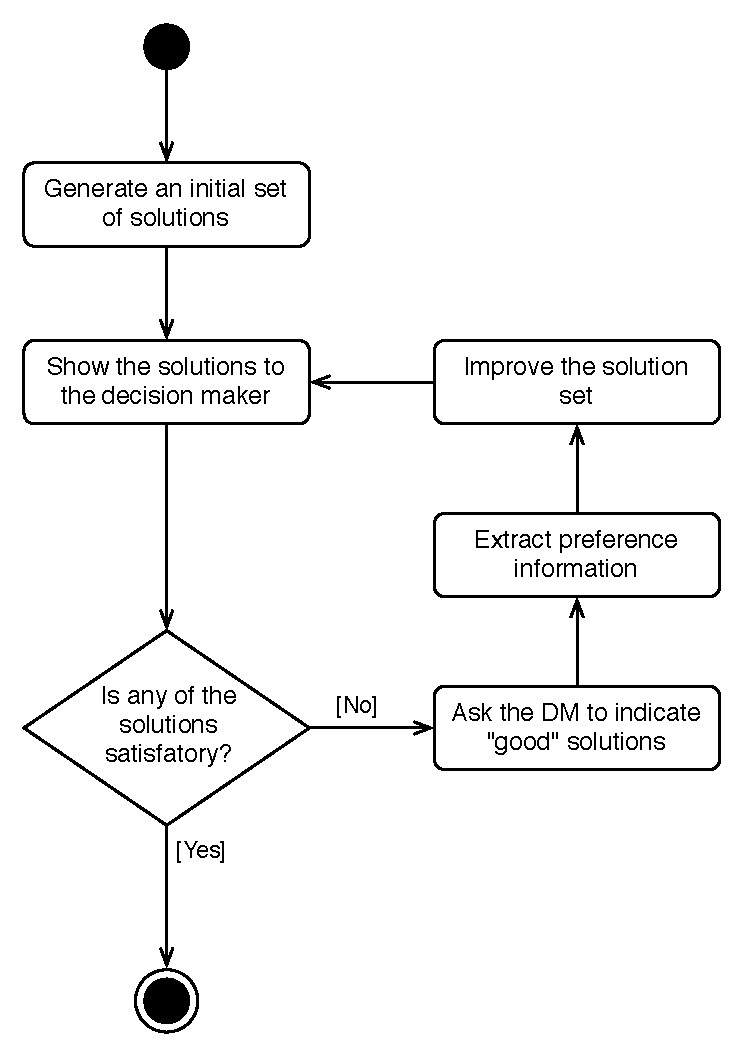
\includegraphics[scale=0.65]{img/imoprocess_uml}
  \caption{An activity diagram for a typical interactive process}
  \label{imoprocess_uml}
\end{figure}

From the DM's answers a preference model is built. This additional preference
information guides the search towards a~region indicated by the Decision
Maker. This can save the computational cost, because the algorithm doesn't
have to go through the whole search space.

Again, new solutions, probably better fitted to the DM's preferences are
generated and the algorithm shows them to him or her. If he or she finds it
satisfactory (or a~stop condition is met) then the algorithm stops. Otherwise
it advances to the next iteration.

There are several types of the IMO methods (consult~\cite{MRW08} for an
in-depth description):
\begin{itemize}
\item \textbf{Trade-off based methods}. A~trade-off is an exchange, a price that
  one is willing to pay (in form of lost on some of the criteria), in order to
  benefit on another criterion (or criteria). These methods ask the DM
  questions about the trade-offs he or she can accept and then, a~preference
  model is inferred based on the tread-offs.
\item \textbf{Reference point approaches} --- the DM specifies bounds on
  values of the objective functions (i.e. reference points) and then, he or
  she can observe the effect of the bounds on the generated solutions.
\item \textbf{Classification-based methods}. It is not possible to improve a
  value of a goal of a solution from the Pareto-frontier without worsening
  other goals of the solutions. In the classification-based methods the DM is
  asked to select goals that can be impaired and the ones that he or she wants
  to improve.
\end{itemize}

The interactive approach requires the Decision Maker's collaboration during
the process, however the approach offers strong benefits to justify this
dedication. Clearly, the computational cost required is lower than in other
approaches, because there is no need to evaluate whole solution space, just
its small subset. The DM may not be able to express a~global structure of his
or her preferences up front. It is also possible that his or her preferences
will change along with the change in understanding of the problem. During the
interactive process the DM has an immediate feedback --- he or she may see how
the decisions are affecting problem solutions.

One can say that solving a Multi-Objective Optimization problem is a
constrictive process, where the Decision Maker learns more about the problem
--- what kind of solutions are possible and how his of her choices influences
the results (see~\cite{MRW08}). As a result, not only the most preferred
solution is given, but also the problem understanding by the DM is better.


\section{Evolutionary Approaches to MOO}
\label{sec_ea_in_moo}

\begin{figure}
  \centering 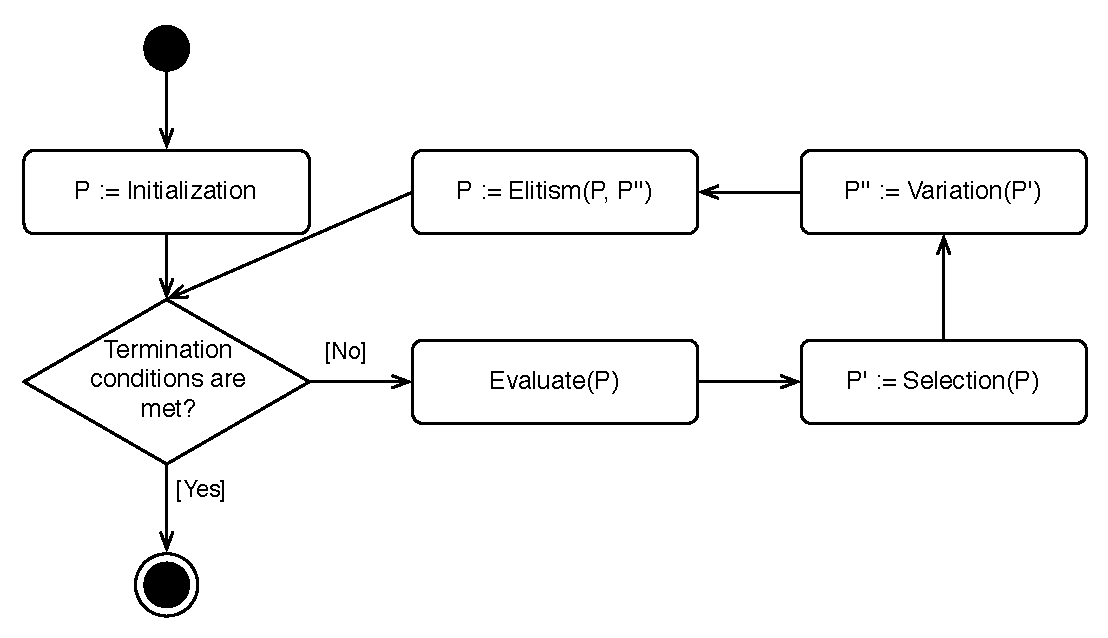
\includegraphics[scale=0.65]{img/eo}
  \caption{An evolutionary optimization procedure}
  \label{eo}
\end{figure}

In 1859, Charles Darwin published his work ``On the origin of
species''~\cite{Dar1859}. He introduced a~scientific theory describing the
evolution of species through the process called natural selection.  According
to the theory, a trait can become less or more common in the population in
dependence on its effect upon the survival and reproduction of the individuals
bearing the trait.

This idea can be easily transfered to the optimization field. A~solution to
a~problem --- that is, the set of values of problem's decision variables ---
is a~single individual in the population. The problem is the environment ---
the higher the solution evaluation on a~given problem, the better it is fitted
to the environment. A~better fitness means higher chance that the traits of
a~solution will be present in the next iteration (an analogue of
a~reproduction success rate). First successful applications of the idea were
done in the electrical engineering field (see~\cite{Fog64}) and in the fluid
mechanics (see~\cite{Rec65, Sch65}).

The main differences between the classical and the evolutionary optimization
(EO) are (see~\cite{Deb08}):

\begin{itemize}
\item \textbf{Population-based}. An EO procedure uses a~population of
  solutions (a~population approach), whereas the classical algorithms maintain
  one solution at a~time (a~point approach). It enables an algorithm to
  maintain multiple optimal solutions, possibly from different parts of the
  solution space. Unfortunately it rises the memory and computational
  footprint of an EO algorithm.
\item \textbf{Stochastic operators}. An EO procedure uses stochastic operators
  (e.g. selection, crossover or mutation) instead of deterministic ones.
\item \textbf{Gradient information}. An EO procedure does not usually use
  gradient information directly in performing a~search. This means that the
  procedure is immune to local optima in a~search space. However, the EO
  procedure may not be competitive with dedicated gradient approach.
\end{itemize}

The basic evolutionary optimization procedure is shown in Figure~\ref{eo}. The
algorithm starts with creating a~population of solutions. Usually the
population is created at random within bounds of decision variables. Then
a~succesion of generations starts. The populations is updated by a~sequence of
operators.

First, the population is evaluated. The evaluation means establishing an
relative preference order, that is sorting solutions from the best to the
worst. After the evaluation the algorithm chooses solutions to fill the mating
pool. The better the solution the higher the probability to be chosen. Then,
the variation operator is being used. It is a series of steps, such as
crossover or mutation, generating a~succeeding generation (an offspring) from
parents in the mating pool. The crossover ensures that parents' traits will be
present in the next generation while the mutation acts as local search in the
solution's neighborhood. Finally, the elitism operator combines the old
population with the newly created offspring. Coping best solutions from the
former ensures the algorithm has a monotonically non-degrading value of the
best solution.

\begin{figure}
  \centering 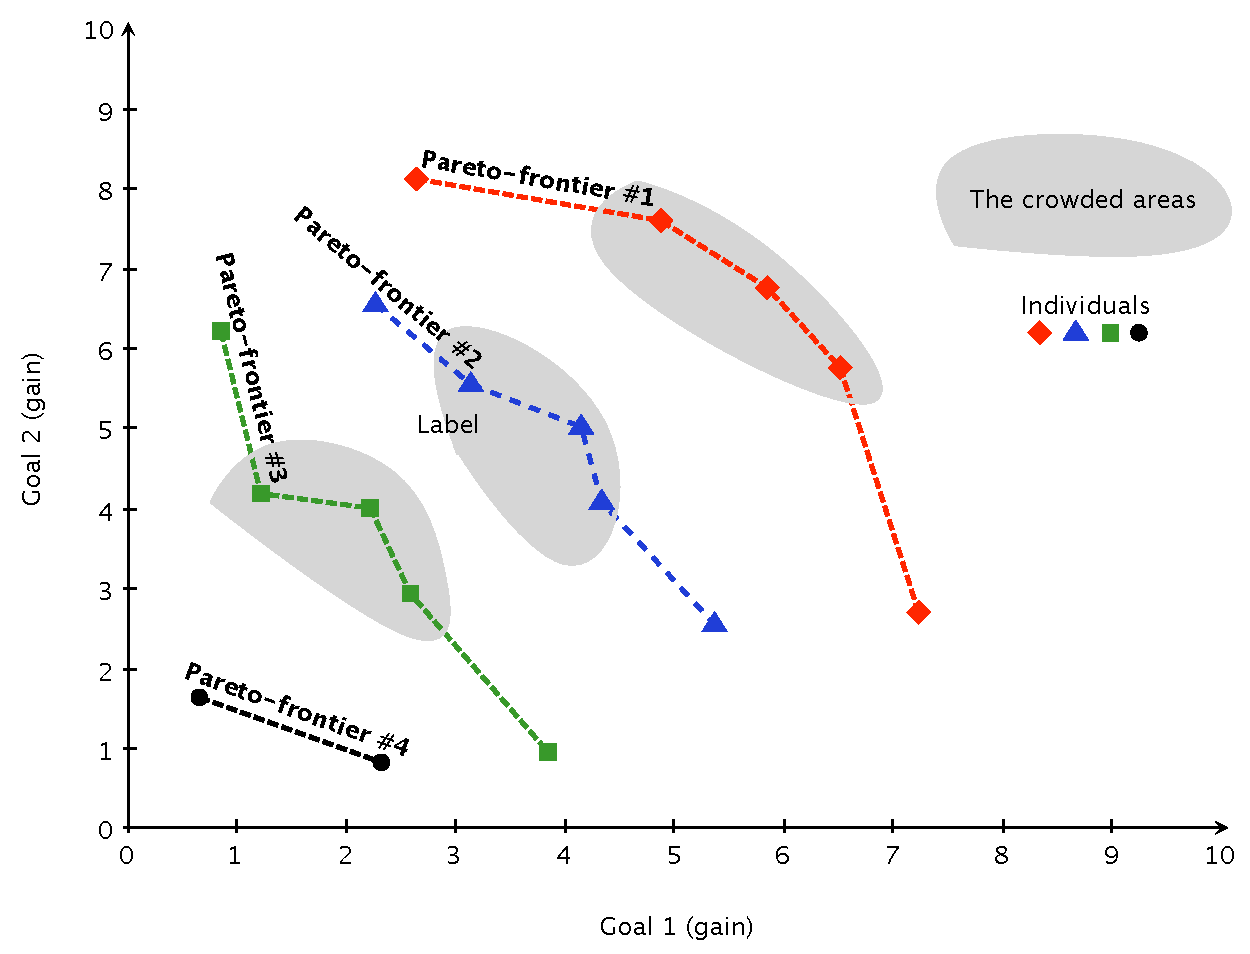
\includegraphics[scale=0.55]{img/nsga}
  \caption{The NSGA-II evaluation}
  \label{nsga}
\end{figure}

The choice of a~fitness function is critical to the algorithm's
performance. In case of a~problem with a~single criterion this is trivial ---
a~value of the goal can be used. However, in the case of the Multi-Objective
Optimization, there are a number of objective functions to be
optimized. A~possible approach to the problem is to use the dominance
principle (\cite{Gol89}):

\vspace{0.5cm} \textit{A solution x is said to dominate the other solution y,
  if both of the following conditions are true:}
\begin{enumerate}
\item \textit{The solution x is not worse than y on all objectives. Thus, the
    solutions are compared based on their objective function values.}
\item \textit{The solution x is strictly better than y on at least one
    objective.}
\end{enumerate}

All the solutions that are non-dominated by any other solution are forming the
Pareto-frontier of the problem.

According to~\cite{Deb08} there are two ideal goals of the EMO:
\begin{enumerate}
\item Find a set of solutions which lies on the Pareto-optimal front, and
\item Find a set of solutions which is diverse enough to represent the entire
  range of the Pareto-optimal front.
\end{enumerate}

The most representative example of the Evolutionary Multi-objective
Optimization (EMO) algorithm is NSGA-II (\cite{Deb00}). The basic idea behind
the algorithm is to assign each solution in a~population to a~number of
different Pareto-frontiers. All non-dominated individuals are assigned to
first Pareto-frontier and then removed from the population. All non-dominated
individuals after the removal are then assigned to second frontier. The
process repeats until there are individuals in the population. The lower the
number of the~frontier, which an individual belongs to, the higher the fitness
function for it. In case of a~tie the crowding score is taken into account ---
the lesser the crowd in the solution's neighborhood in an objective space, the
better the solution's evaluation. This is illustrated in Figure~\ref{nsga}.


\section{Dominance-Based Rough Set Approach to MOO}
\label{sec_drsa_in_moo}

A rough set is an approximation of a~conventional set --- a pair of sets being
a~lower and an upper approximation of the original set (\cite{Paw82}). The
lower approximation is a~set of all objects that unambiguously can be
classified as members of the target set. On the other hand, the upper
approximation is a~set containing objects that cannot be unambiguously
classified as members of the complement of the target set.  A~boundary region
is the part of solution space being part of the upper approximation, but not
the lower one.

\begin{figure}
  \centering 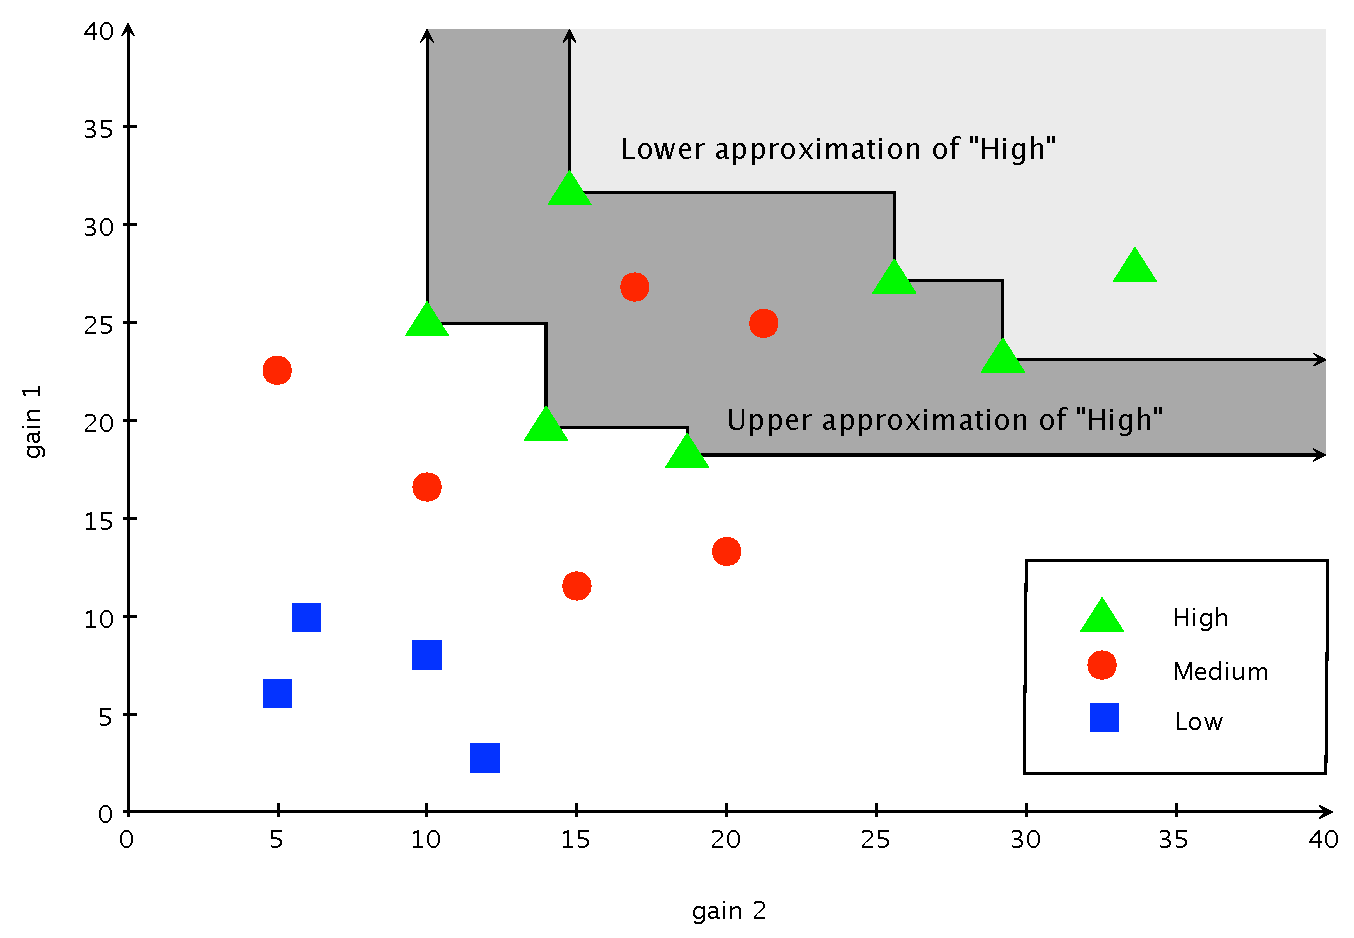
\includegraphics[scale=0.5]{img/drsa}
  \caption{An example of the DRSA approach}
  \label{drsa}
\end{figure}

Dominance-based Rough Set Approach (DRSA) is an extension of the rough set
theory introduced in~\cite{GMS01, GMS02, GMS05}. The indiscernibility relation
is replaced by the dominance relation (defined in the former section). DRSA is
applicable in the decision support field.

DRSA can model the situations in which a~finite set of objects --- vectors of
values in the decision variable space --- has been classified to some decision
classes, such that one object belongs to exactly one class. The classes are
preference ordered. The main task of DRSA is to structure the classification
into lower and upper approximations of unions of ordered decision classes,
prior to induction of monotonic decision rules, representing the preferences
of an agent who made the classification decision. An example of the DRSA data
structuring is given in Figure~\ref{drsa}.

The data in Dominance-based Rough Set Approach are often presented in
a~decision table. The objects being considered are written in table rows, the
decision attributes are table columns. The last column is classification of
the objects to a decision classes. A formal definition of the decision table
can be easily found in the literature. An example is given in
Table~\ref{t:dec_tab-example}.

\begin{table}
  \centering
  \begin{tabular}{c c c c | c}
   \hline
   Student & Mathematics & Physics & Literature & Overall class \\
   \hline
   \hline
   1 & good & medium & bad & bad \\
   2 & medium & medium & bad & medium \\
   3 & medium & medium & medium & medium \\
   4 & medium & medium & medium & good \\
   5 & good & medium & good & good \\
   6 & good & good & good & good \\
   7 & bad & medium & medium & bad \\
   8 & bad & bad & medium & bad \\
   \hline
  \end{tabular}
  \caption{An example of the decision table}
  \label{t:dec_tab-example}
\end{table}

On the basis of the table, decision rules may be induced. They are generalized
description of the knowledge represented in the table. A~decision rule is a
Horn clause (see~\cite{Hor51}) in form of \textit{``if~..., then~...''}. The
former part is called \textit{condition} and the latter ---
\textit{consequent}. The condition part compares a~value of an object
attributes with given thresholds and the consequent part represents the object
classification if the condition part holds. Rules can be either
\textit{certain} --- based on objects from the lower approximation of the
class, \textit{possible} --- based on objects from the upper approximation and
\textit{approximate} --- based on the boundary region. Each decision rule
should be minimal, i.e. cardinality of the set of conditions should be
minimal.

Example rules generated from Table~\ref{t:dec_tab-example} are as follows:
\begin{enumerate}
\item If \textit{Literature $\ge$ good} then \textit{Student $\ge$ good},
\item If \textit{Mathematics $\le$ bad} and \textit{Physic $\le$ medium} then
  \textit{Student $\le$ bad},
\item If \textit{Mathematics $\ge$ medium} then \textit{Student $\ge$ medium}
  (possible).
\end{enumerate}

DRSA can handle uncertainty and contradictions in the data, thus it can model
a~wide class of real-world decision problems. For each rule $r$ given in from
$\Phi \to \Psi$, the following measures are defined:
\begin{itemize}
\item Support: $\textit{supp}(\Phi, \Psi) = \textit{cardinality}(||\Phi \land
  \Psi||)$ --- is the number of objects for which the condition of the rule
  holds and the object classification is consistent with the consequent of the
  rule.
\item Confidence: $\textit{confidence}(\Phi, \Psi) =
  \dfrac{\textit{supp}(\Phi, \Psi)}{\textit{cardinality}(||\Phi||)}$ --- is
  the number of objects supporting the rule in a~relation to the number of
  objects for which the rule's condition holds.
\end{itemize}.

Objects supporting rule no.~3  are \{S2, S3, S4, S5\}, but the condition part
holds also for S1. The support is thus: $\textit{supp}(r_3) = \frac{4}{5} = 0.8$.

To induce all rules from the decision table one can use the All Rules algoritm
(an optimized version is described in~\cite{Zur01}). Another option is to use
the DomLem algorithm (\cite{GMS+01}) generating a~minimal set of rules
covering all the objects from a given table.


%%% Local Variables: 
%%% mode: latex
%%% TeX-master: "main"
%%% End: 
